\subsection{User-defined Functions}

As your code becomes longer, 
you will start to realize that similar processing or 
calculation appears several times in a macro or through macro sets. 
To simplify such redundancy, one could write a 
separate \ilcom{function} that works as a module for macros. 
For example, if you have a simple code like:
\lstinputlisting[morekeywords={*,}]{code/code15.ijm}
It should be easy for you to expect that this macro will print out "3" in the Log window. 
From this macro, we could extract part of it and make a separate function. 
\lstinputlisting[morekeywords={*,}]{code/code15_1.ijm}
This is not a macro, but is a program that works as a unit. 
Functions can be embedded in macro. \ilcom{ReturnAdd }(code 15.1) is the name of the function, 
and the following \ilcom{(n, m)} are the variables that will be used in the function. Within the function, 
n and m will be added and the result of which is substituted in to a new variable p. 
\ilcom{return p} in line 4 will return a value as an output of the function. 
We call such custom-made function as ``user-defined function''. Using this function, code 15 can be rewritten as
\lstinputlisting[morekeywords={*,}]{code/code15_2.ijm}
or simpler, by nesting the custom made function inside ImageJ native function \ilcom{print()},
\lstinputlisting[morekeywords={*,}]{code/code15_3.ijm}
Macro interpreter reads the macro line by line. When the interpreter sees \ilcom{ReturnAdd(a, b)}, 
the interpreter first tries to find the function within the ImageJ Build-in function. 
If its not there, the interpreter looks for the function within the same macro file\ldots 
(user-defined function (e.g. \ilcom{ReturnAdd(a, b)} must be written in the same macro file. 
Here is how it looks like: a macro that uses a function. 
%figure
\begin{figure}[htbp]
\begin{center}
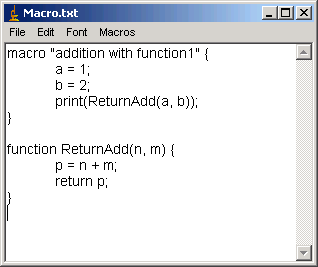
\includegraphics[scale=0.6]{fig/fig2411_usingFunction.png}
\caption{A macro file with function}
\label{fig:MacroWithFunction}
\end{center}
\end{figure} 

In this simple case, 
you might not feel the convenience of the user-defined function, 
but you will start to feel its power as you start writing longer codes. 
Advantages of using \ilcom{function} are
\begin{enumerate} 
\item Once written in a macro file, it could be used as a single line function 
as many times as you want in the macro file. This also means that if there is a bug, 
fixing the function solves the problem in all places where the function is used.
\item Long codes could be simplified to an explicit outline of events. Such as:
\begin{lstlisting}[numbers=none]
macro "whatever" {
    	function1;
		function2;
		function3;
}
\end{lstlisting}
\end{enumerate}
